\par Robots can be broadly classified into two categories: serial and parallel. Serial robots are distinguished by a series of linked joints, whereas parallel robots are characterized by multiple axes that move in parallel, typically working in unison to support a single platform.

\par Parallel robots represent a significant branch in the field of robotics due to their precision and versatility in various applications, including pick-and-place manipulation, simulators, manufacturing, and tooling, among others. As described in \cite{shao2024}, these applications encompass both industry and medicine, capitalizing on the high rigidity, precision, and speed of these robots to compensate for the performance limitations of serial robots.

\par The origin of parallel robots can be traced back to the 1960s, with the development of the Gough-Stewart \cite{stewart1965} parallel mechanism (Figure \ref{fig:stewart_platform}), which has become one of the most iconic in the field of parallel robotics. Subsequently, in the 1980s, Reymond Clavel devised a robust parallel structure comprising three translational degrees of freedom and one rotational degree of freedom, as depicted in Figure 2. The Delta Robot has become one of the most significant examples in the field of parallel robotics. 

% https://www.weiss-world.com/Productpics/handling/Pick%20%26%20Place/DR/dr.png
% https://actu.epfl.ch/news/the-delta-robot-swiss-made-and-fastest-in-the-worl/
% {stewart1965}
\begin{figure}
    \centering
    \begin{subfigure}[t]{0.45\textwidth}
        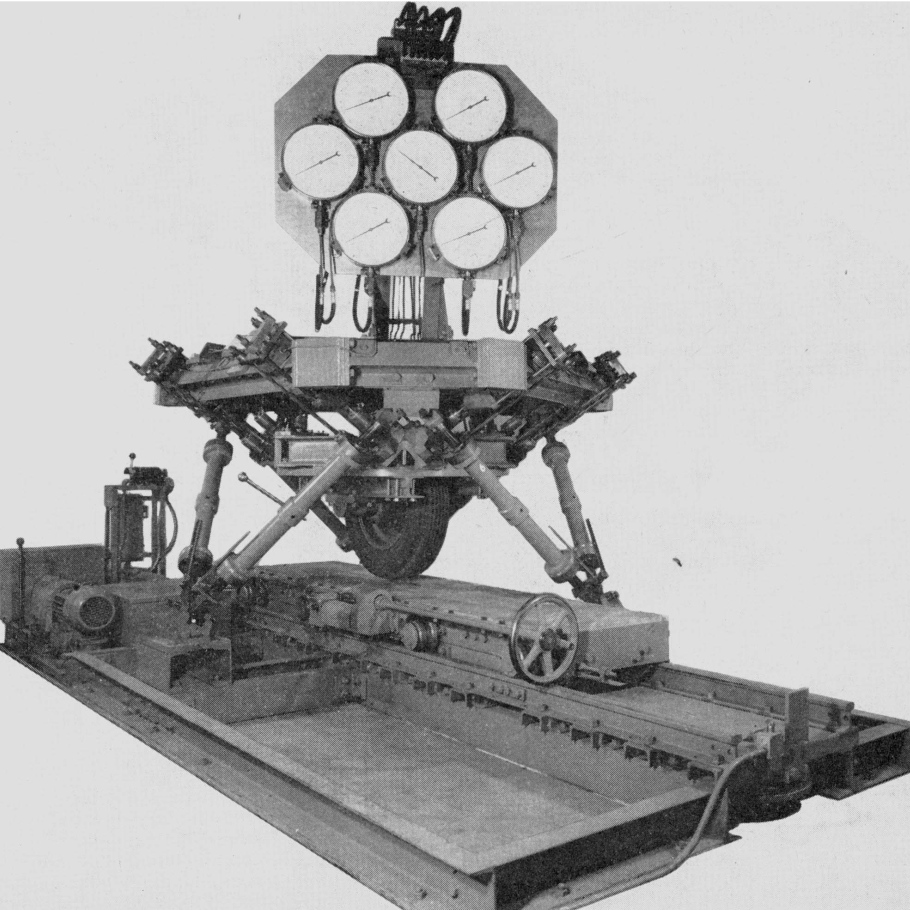
\includegraphics[width=\textwidth]{stewart_platform}
        \caption{Gough-Stewart Platform}
        \caption*{Source: Adapted from \cite{stewart1965}}
        \label{fig:stewart_platform}
    \end{subfigure}
    \begin{subfigure}[t]{0.45\textwidth}
        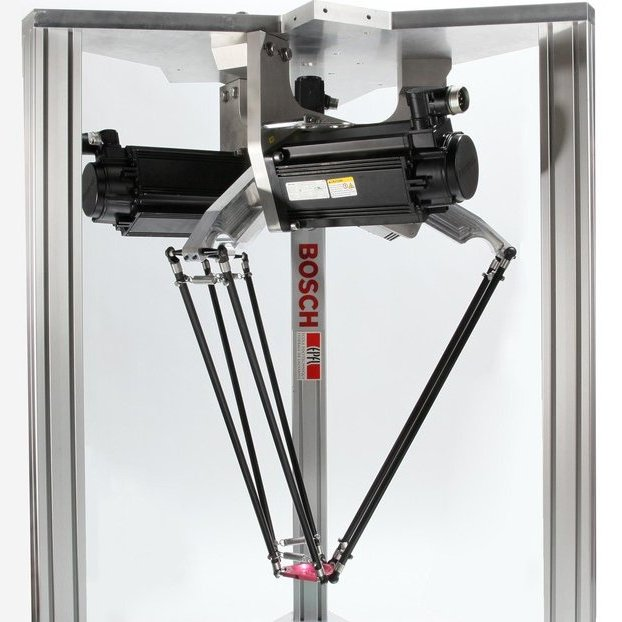
\includegraphics[width=\textwidth]{clavel_robot}
        \caption{Clavel's Delta Robot}
        \caption*{Source: Adapted from \cite{sandyEFPL}}
        \label{fig:delta_robot}
    \end{subfigure}
    \caption{Traditional parallel robots}
    \label{fig:traditionals}
\end{figure}

\par Another distinguishing feature of these robots is the presence of multiple closed kinematic chains that connect and move the mobile platforms. In contrast, to serial robots, which operate with an open kinematic chain and move in a linear sequence. Nevertheless, according to Briot and Kahrs \cite{briot2023}, the fundamental questions about this class of robots have been addressed. As a result, there has been a shift in interest towards exploring new alternatives in parallel robots in recent years.

\par The current research in robotics transcends conventional definitions, pushing the boundaries of this field and fostering new possibilities and innovations. Briot and Kahrs \cite{briot2023} illustrate how parallel manipulators have been integrated into various novel robot types, such as continuum robots, flying robots, cable-driven robots, underactuated robots, multi-fingered hands, and microscale parallel robots. However, this emerging class of robots presents significant scientific challenges in the design, modeling, and control of these systems. Among these categories, aerial robots, parallel robots, and continuum or soft robots are particularly noteworthy for their ability to venture into new areas due to their lightness and flexibility.

\par Building upon these insights, Russo et al. \cite{russo2023} offer a comprehensive review that addresses recent advancements, current limitations, and ongoing challenges in the design, modeling, and control of continuum robots. Continuum robots are classified according to their design, with distinction made between extrinsic and intrinsic actuation methods. Extrinsic actuation (Figure \ref{fig:extrinsic_continuum_robots}) involves transmitting motion from the robot's base along its structure. This is categorized into three main families depending on the transmission elements used: tendon-driven, concentric tube (Figures \ref{fig:concentric_tube}, \ref{fig:concentric_tube_ex}), and rod-driven robots (Figures \ref{fig:rod_driven}, \ref{fig:rod_driven_ex}). Moreover, robots with intrinsic actuation utilize actuators within their structural framework to produce motion, thereby enabling actuation to occur within the robot's body.

\begin{figure}
    \centering
    \begin{subfigure}[b]{0.4\textwidth}
        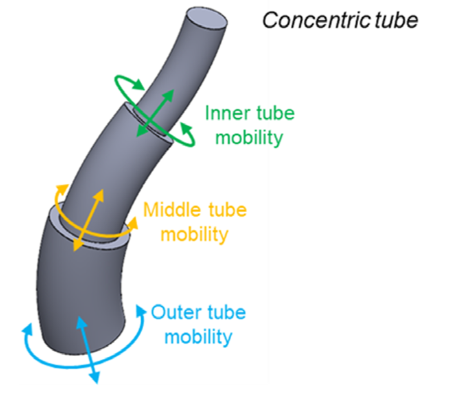
\includegraphics[width=\textwidth]{concentric_tube}
        \caption{Concentric tube robot mobility}
        \label{fig:concentric_tube}
    \end{subfigure}
    \begin{subfigure}[b]{0.4\textwidth}
        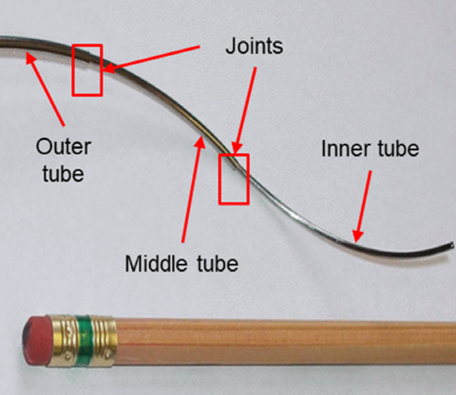
\includegraphics[width=\textwidth]{concentric_tube_example}
        \caption{Concentric tube prototype}
        \label{fig:concentric_tube_ex}
    \end{subfigure}
    \vskip\baselineskip
    \begin{subfigure}[b]{0.4\textwidth}
        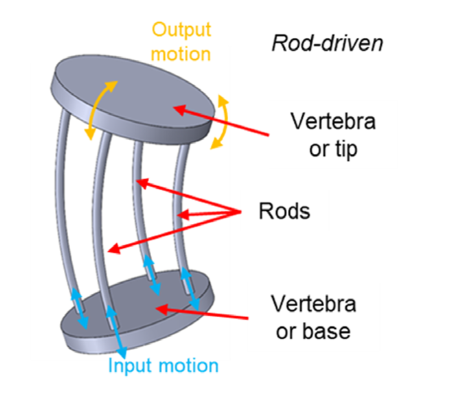
\includegraphics[width=\textwidth]{rod_driven}
        \caption{Rod-driven continuum robot conceptual scheme}
        \label{fig:rod_driven}
    \end{subfigure}
    \begin{subfigure}[b]{0.4\textwidth}
        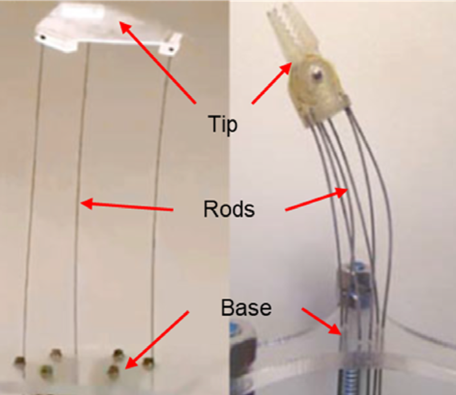
\includegraphics[width=\textwidth]{rod_driven_example}
        \caption{Parallel continuum rod-driven robot prototype}
        \label{fig:rod_driven_ex}
    \end{subfigure}
    \caption{Continuum robots with extrinsic actuation}
    \caption*{Source: Adapted from \cite{russo2023}}
    \label{fig:extrinsic_continuum_robots}
\end{figure}



\par The current challenges in the field of parallel continuum robot design and modeling include improving through the miniaturization of actuators, the integration of these robots with rigid ones, the exploration of smart materials, the accurate modeling of environments, and the implementation of proprioception with new sensors \cite{russo2023}. Additionally, modeling efforts are focused on representing interaction environments and improving real-time implementations, as well as standardizing simulation environments. Control challenges include ensuring precise manipulation and adapting to dynamic environments using advanced sensor technology and adaptive strategies

\par This project aims to address the efficiency challenges of continuum robots by miniaturizing their parallel linear actuators. Specifically, the project focuses on the implementation of adaptive control strategies for various applications using an extrinsic actuation platform for rod-driven continuum robots. This research aims to improve affordability and ease of use in order to facilitate broader adoption and usability in practical contexts.


\section{Objectives}

\subsection{General Objective}
Design and develop a portable, modular, and scalable platform with a control system for the actuation of rod-driven continuum parallel robots.

\subsection{Specific Objectives}
\begin{itemize}
    \item Adapt an existing design of a rod-driven continuum parallel robot, with the goal of reducing its size while maintaining its functionality and performance.
    \item Design linear actuators that provide precise control and enable dexterous movements, ensuring high accuracy and reliability.
    \item Fabricate all necessary components and assemble a fully functional physical prototype of the platform, adhering to the design specifications.
    \item Implement a customized language specification for programming the linear actuators, allowing for tailored control and flexibility in operations.
    \item Develop an application to interface with the control system, utilizing the created protocol to facilitate seamless communication and control.
    \item Conduct comprehensive experimental testing and validation of the system, ensuring it meets all performance criteria and operational standards.
\end{itemize}